%!TEX root = ../../thesis.tex

\section{Exploiting overlap between distributions}
\label{chapter:limitations:overlap}

Recent works have explored the use of brain signals to directly control virtual and robotic agents in sequential tasks. So far in such brain-computer interfaces (BCIs), an explicit calibration phase was required to build a decoder that translates raw EEG signals from the brain of each user into meaningful feedback signals.
%
This paper proposes a method that removes the need for such a calibration phase, and allows a user to control an agent to solve a sequential task.
%
The proposed method assumes a distribution of possible tasks, and infers the interpretation of EEG signals and the task by selecting the hypothesis which best explains the history of interaction. 
%
Also, we use a measure of uncertainty of the task and of the EEG signal interpretation as an exploratory reward for a planning strategy, and this speeds up learning by guiding the system to regions that help disambiguate among task hypotheses.
%
We report experiments where four users control, by means of a BCI, an agent on a virtual world to reach a target without any previous calibration process.

examplify here the work of AAAI with the bhattacharrya method


For the planning we use it on the sexpected signal as describe in plaing blabal

Computing the similarity between two Gaussian distributions for all state-action pairs was not feasible in real time. In order to improve computation efficiency we do not rely on a precise metric between Gaussian distributions and only consider the similarity between their means (empirical tests did show that this approximation does not impact the results).


EEG-based brain-computer interfaces (BCI) have been used successfully to control different devices, such as robotic arms and simulated agents, using self-generated (e.g. motor imagery) and event-related potentials signals (see \cite{millan10} for a review). 
%
Error-related potentials (ErrPs) are one kind of event-related potential that appears when the user's expectation diverges from the actual outcome \cite{Falkenstein00}. Recently, they have been used as feedback signals for devices to solve a user's intended task \cite{chavarriaga2010learning,iturrate13}.

As in most BCI applications, ErrP-based BCIs require a calibration phase to learn a decoder (e.g. a classifier) that translates raw EEG signals from the brain of each user into meaningful feedback signals. This calibration is required mainly due to several characteristics of the EEG signals, such as their non-stationary nature \cite{vidaurre11}; the large intra- and inter-subject variability \cite{Polich1997}, and the variations induced by the task \cite{iturrate2013task}. The presence of an explicit calibration phase, which length and frequency is hard to tune and is often tedious and impractical for users, hinders the deployments of BCI applications out of the lab and thus calibration free methods have been identified as an important step to apply this technology in real applications \cite{millan10}.

Despite the importance of calibration-free BCIs, there are few BCI applications that are able to calibrate themselves during operation. For long term operation using motor rhythms, it is possible to adapt the decoder online \cite{vidaurre2010towards}. In invasive BCIs, Orsborn et al. proposed a method to learn from scratch in closed loop a decoder for known targets using pre-defined policies to each target \cite{Orsborn2012}. However, the approach needed for a warm-up period of around 15 minutes. For P300 spellers, Kindermans et al. proposed a method to auto-calibrate the P300 detector by exploiting multiple stimulations and prior information \cite{Kindermans2012a,Kindermans2012b,tangermann2013zero}. They particularly exploit the fact that the speller paradigm guarantees that only one event out of fixed number (e.g. one out of six) encodes a P300 potential. In our setup it is however impossible to define a sequence of actions that guarantee a specific ratio of label in the received signals.


\cite{kindermans2014integrating}, they merge most of the method they have been developing.
\begin{itemize}
    \item Dynamic stopping, where the system stop when it reaches a confidence threshold.
    \item Language model as a prior probability on next letter
    \item Transfer learning where a model of previous subjects is used to ``regularizes the subject-specific solution towards the general model.''
    \item Unsupervised learning (that is the EM approach we refer to when citing their work)
\end{itemize}

\cite{schettini2014self} continuous adaptation of the classifier model, a first session using a calibration procedure, and on latter run, the system re-calibrate itself continuously.


Our main contribution is a BCI method without any explicit calibration phase that simultaneously and seamlessly infers a decoder of EEG error-related potentials while controlling a device to achieve a sequential task.

The core idea of the method is to assume a distribution of possible tasks, and infer the interpretation of EEG signals and the task by selecting the hypothesis which best explains the history of interaction. In what follows, we will use the term ``virtual label'' or ``label'' to denote the interpretation of a given EEG signal as a feedback signal (e.g. ``correct'' or ``wrong''). Considering that, for a particular task hypothesis provides, we can infer the labels that should be provided by the user in each state of the task, thus, given a particular interaction history, it is possible to compute a different EEG decoder for each task hypothesis. As the correct task assigns the correct labels to the EEG signals, the hypothesis which provides the decoder with best classification accuracy and compactness can then be selected as the most probable. Since the process is iterative, this inference can be continuously run and updated as new data comes in, which removes the need for an explicit calibration.

This method is inspired from our previous work \cite{grizou2013robot} which considered a robotic setting and speech utterances as feedback signals. In this work we improved the algorithm formalism, the robustness to noisy high-dimensional signals (e.g.\ EEG), and show that it is possible to use model-based planning based on the uncertainty about the tasks and the feedback signals to explore the space efficiently while learning.

We also present an evaluation of this method with online experiments with four users who control an agent in a virtual world. The results show that the proposed method is able to learn good feedback models and solve the task efficiently without any explicit calibration. Offline experiments show that our unsupervised trained decoder achieves similar performances than calibration based systems and illustrate the benefits of our planning strategy for speeding up learning.

\subsection{BCI control based on feedback signals}

BCI control based on feedback signals differs from classical brain-computer interfaces in the sense that the user does not actively deliver commands to the device, but only delivers feedback about actions performed by the device \cite{chavarriaga2010learning,iturrate13}. In this setting, the device needs to actively execute actions to solve the task and to be able to learn an intelligent behavior from the feedback. This idea can be seen as a shared control strategy \cite{millan10}, where both the user and the device help each other to solve a task.

Essentially, this BCI control follows an iterative sequential process where the device performs an action and the user assesses the action. This assessment will elicit potentials into the user's brain that can be recorded using EEG and will be different for correct and wrong assessments. The potentials elicited in the user's brain after performing assessments are called error-related potentials, signals generated when the user observes a device performing a wrong action \cite{FerrezErrores}. After a calibration phase and once a usable decoder of these signals is available, user's assessments can be translated into (normally binary) feedback, which the device can use to learn a task and adapt its behavior. 
%
This control based on user's assessments decoded from brain signals can be exemplified for a reaching task, where the user wants to reach a target position unknown by the system (see Figure \ref{fig:GM} Top). The device performs several discrete actions (e.g. moving left or right), and learns from the feedback given by the user. After several steps, as the meanings of the signals are known, the device can infer which is the user's desired position and how to reach it. The following section explain how we can achieve similar performance without knowing the brain signal decoder beforehand.

\subsection{Method}


\subsection{Control task}
We consider a 5x5 grid world, where an agent can perform five different discrete actions: move up, down, left, right, or a target-reached action. The user goal is to teach the agent to reach one, yet unknown to the agent, of the $25$ discrete states which represent the set of possible tasks (i.e. one task per possible target state). We thus consider that the agent has access to 25 different task hypotheses. We use \textit{Markov Decision Processes} (MDP) to represent the problem \cite{sutton1998reinforcement}. From a given task $\xi$, represented as a reward function, we can compute the corresponding policy $\pi_{\xi}$ using, for instance, Value Iteration \cite{sutton1998reinforcement}. 

\subsection{EEG-based feedback signals}

EEG signals were recorded with a gTec system (2 gUSBamp amplifiers) with 32 electrodes distributed according to the 10/10 international system, with the ground on FPz and the reference on the left earlobe. The EEG signals were digitized with a sampling frequency of $256$ Hz, common-average-reference (CAR) filtered and band-pass filtered at $[0.5, 10]$ Hz. 

During operation, the role of the users was to mentally assess the agent's actions as correct or wrong with respect to a selected target, obtaining this way error-related potentials. Previous studies have demonstrated that these signals can be detected online \cite{FerrezErrores}. Following these studies, features were extracted from two fronto-central channels (FCz and Cz) within a time window of $[200,700]$ ms ($0$ ms being the action onset of the agent) and downsampled to $32$ Hz. This leaded to a vector of $34$ features that was the input for our system.

\subsection{Results}

\subsection{Simulated results}

The objective of the offline analysis is to study the impact of our exploration method and evaluate if the classifier learned from scratch with our algorithm can be reused for learning new tasks. Finally we want to evaluate how robust the system is to abrupt changes in the signal properties. For these experiments, to ensure we have sufficient data to achieve statistically significant results, we rely on a large dataset of real EEG data. We used a dataset from \cite{iturrate2013task}, which covers ten subjects that performed two different control problems (denoted $T1$ and $T2$). The role of the users was similar (assess the agent's actions), but the problems differs in the state-action space size and visual representations. For each subject, $T1$ was composed of 1800 assessments, and $T2$ of 1200. Despite the fact that both problems elicit error-related potentials, the EEG signals presented significant differences \cite{iturrate2013task}.

For each subject, and each dataset ($T1$ and $T2$), we simulated $20$ runs of $400$ iterations following the control task. Each time the device performed an action, we sampled the dataset using the ground truth labels corresponding to the correct task and then removed the chosen signal from it. After a first task was identified, and following our approach, we continued running the system to identify new tasks. 

We present most of the results in terms of the quality of the dataset, measured as the classification accuracy that a calibrated brain signal classifier would obtain. Results vary strongly between subjects and we will see that it is a direct consequence of the difficulty of finding a classifier with high accuracy. 

\paragraph{Planning Methods}
We compared the average number of steps (with maximum values of $400$ steps) needed to identify the first task when learning from scratch with different planning methods.

\begin{figure}[!ht]
    \centering
    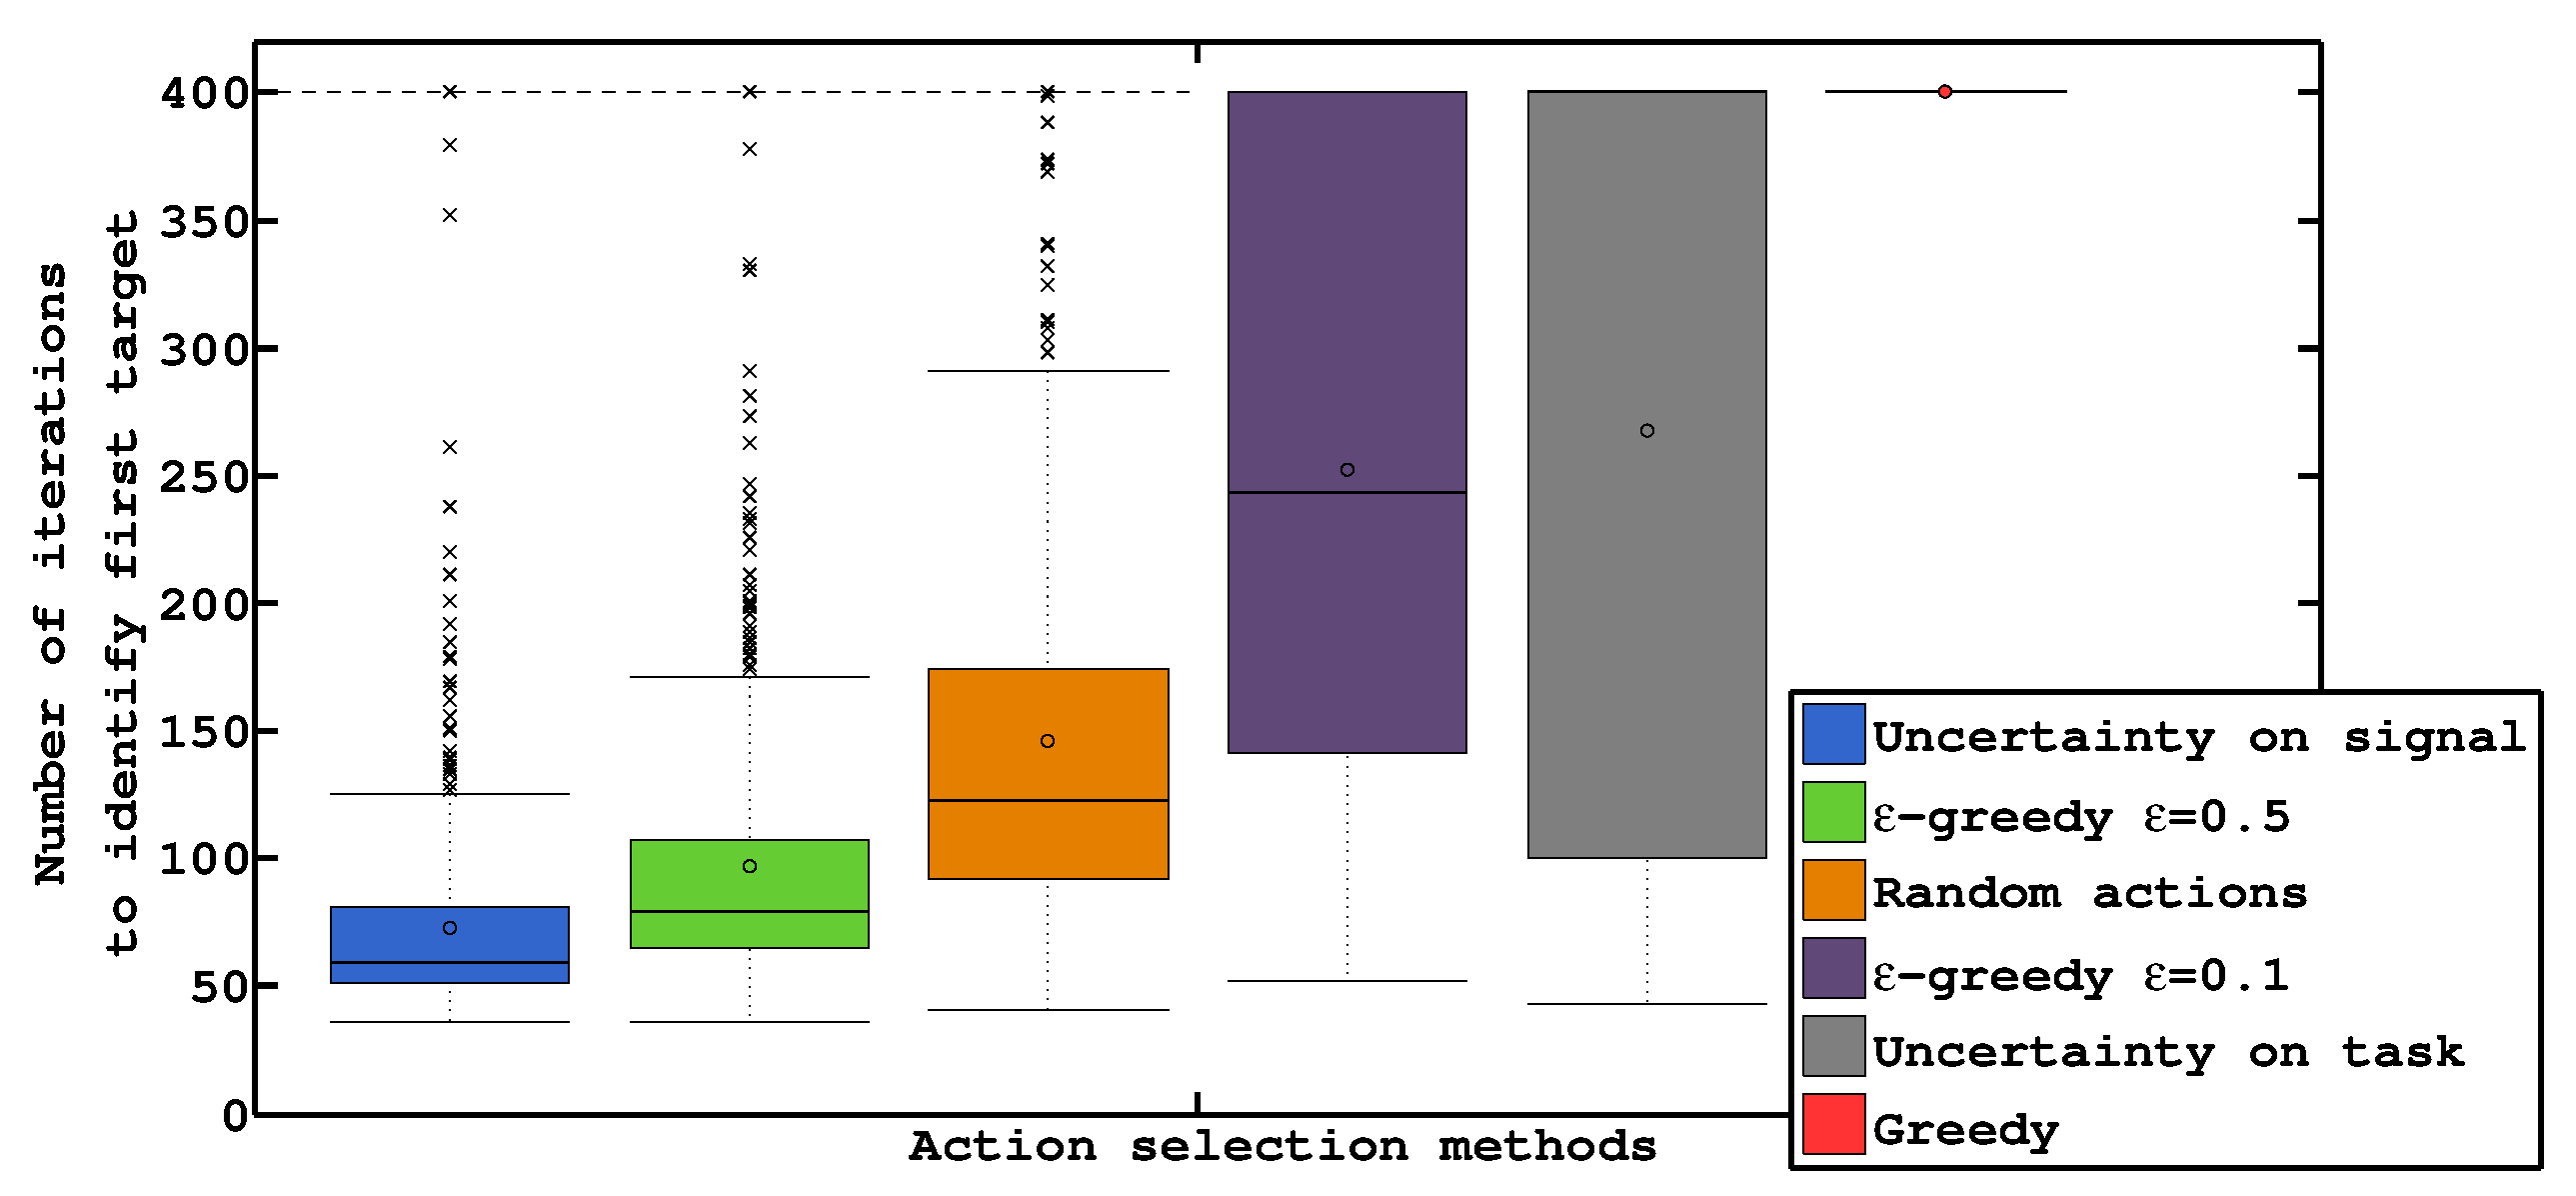
\includegraphics[width=\columnwidth]{\imgpath/battacharyya/plot_planning_first}
    \caption{Comparison of different exploration methods. Our proposed method, based on the uncertainty on the task and the signals interpretation, allows to lead the system to regions that improve disambiguation among hypotheses in a faster way. For the greedy method, all values were $400$ which indicates it never allowed to identify any task.}
    \label{fig:compplan}
\end{figure}

Figure~\ref{fig:compplan} shows the results averaged across subjects, runs and datasets. Values of $400$ means the confidence threshold was not reached after 400 iterations. Our proposed method, based on the uncertainty on the task and the signals interpretation, allows to lead the system to regions that improve disambiguation among hypotheses in a faster way. Trying to follow the most probable task does not allow the system to explore sufficiently (Greedy), and at least some random exploration is necessary to allow a correct identification of the task ($\varepsilon$-greedy). Assessing uncertainty only on the task performs poorly as it does not take into account the signal interpretation ambiguity inherent to our problem. The large variability in the results is mainly due to the large variations in classification accuracy across subjects and datasets. Given these results, the remainder of this section will only consider our proposed planning method.

\paragraph{Online re-estimation of classifier}
After identifying the first task, and following our approach, we continued running the system and measured how many tasks were identified after $400$ steps. The quality of our unsupervised method can be measured according to the percentage of labels correctly assigned (according to the ground truth label), see Figure~\ref{fig:percentageLabels}. In general, having dataset with classification accuracies higher than $75\%$ guaranteed that more than $90\%$ of the labels were correctly assigned. This result shows that our algorithm can also be used to collect training data for calibrating any other state-of-the-art error-related potentials classifier, but has the important advantage of controlling the device at the same time.

\begin{figure}[!ht]
    \centering
        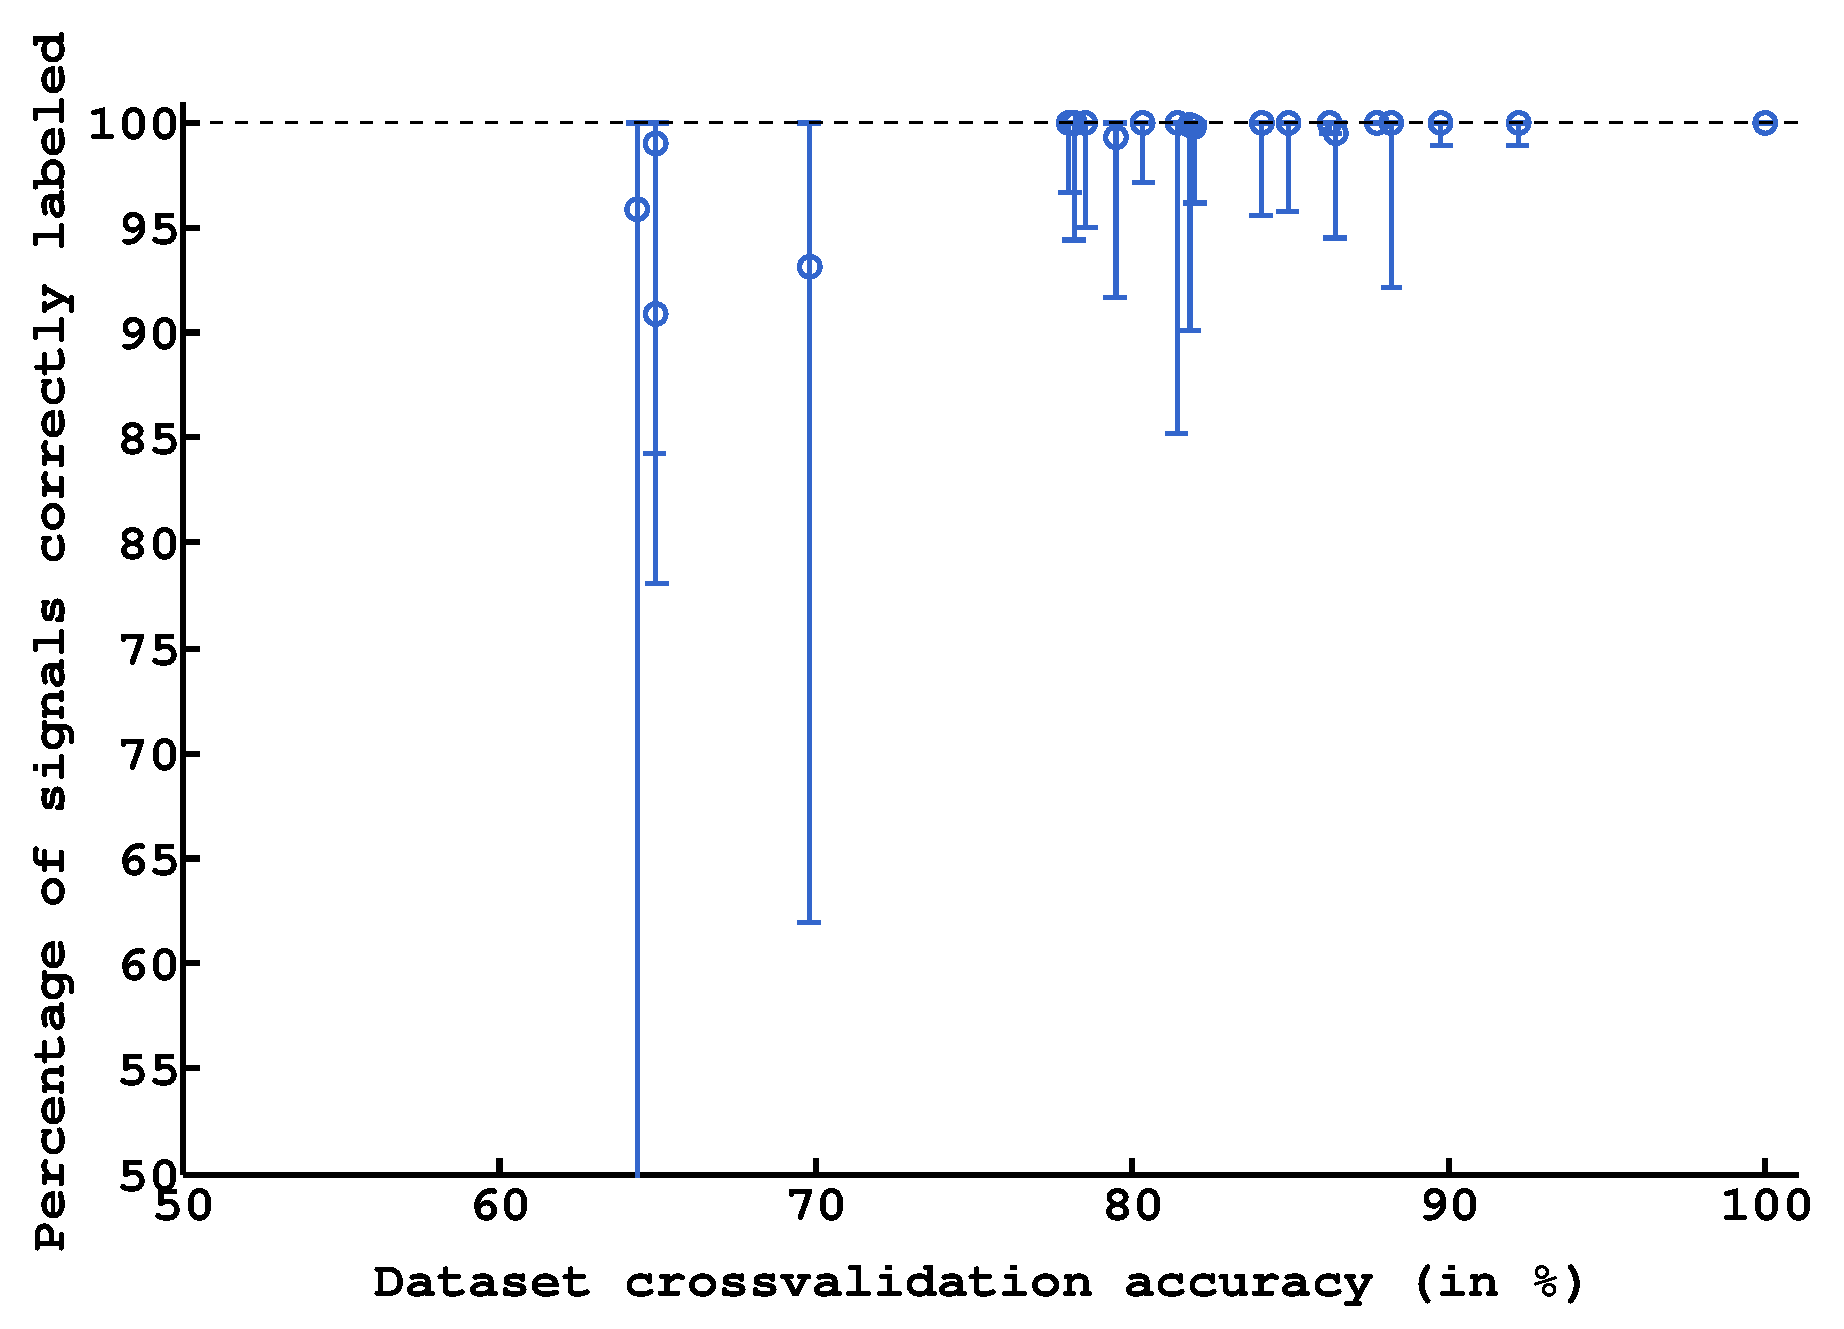
\includegraphics[width=\plotsize\columnwidth]{\imgpath/battacharyya/plot_percent_label}
        \caption{Percentage of labels correctly assigned according to the ground truth label (the markers show the median values and the error bars the $2.5$th and $97.5$th percentiles). In general, having dataset with classification accuracies higher than $75\%$ guaranteed that more than $90\%$ of the labels were correctly assigned.}
        \label{fig:percentageLabels}
\end{figure}

Figure~\ref{fig:bhatta} demonstrates the advantage of switching to a Bayes filter method after identification of a first target instead of keeping the estimation given by the Bhattacharyya coefficient. On the one hand, Bhattacharyya coefficient works very well for small amounts of data because it directly compares model parameters. On the other hand, when there is sufficient data, training a classifier allows for a faster identification since the classifier makes a much harder decision when evaluating a new EEG signal.

\begin{figure}[!ht]
    \centering
        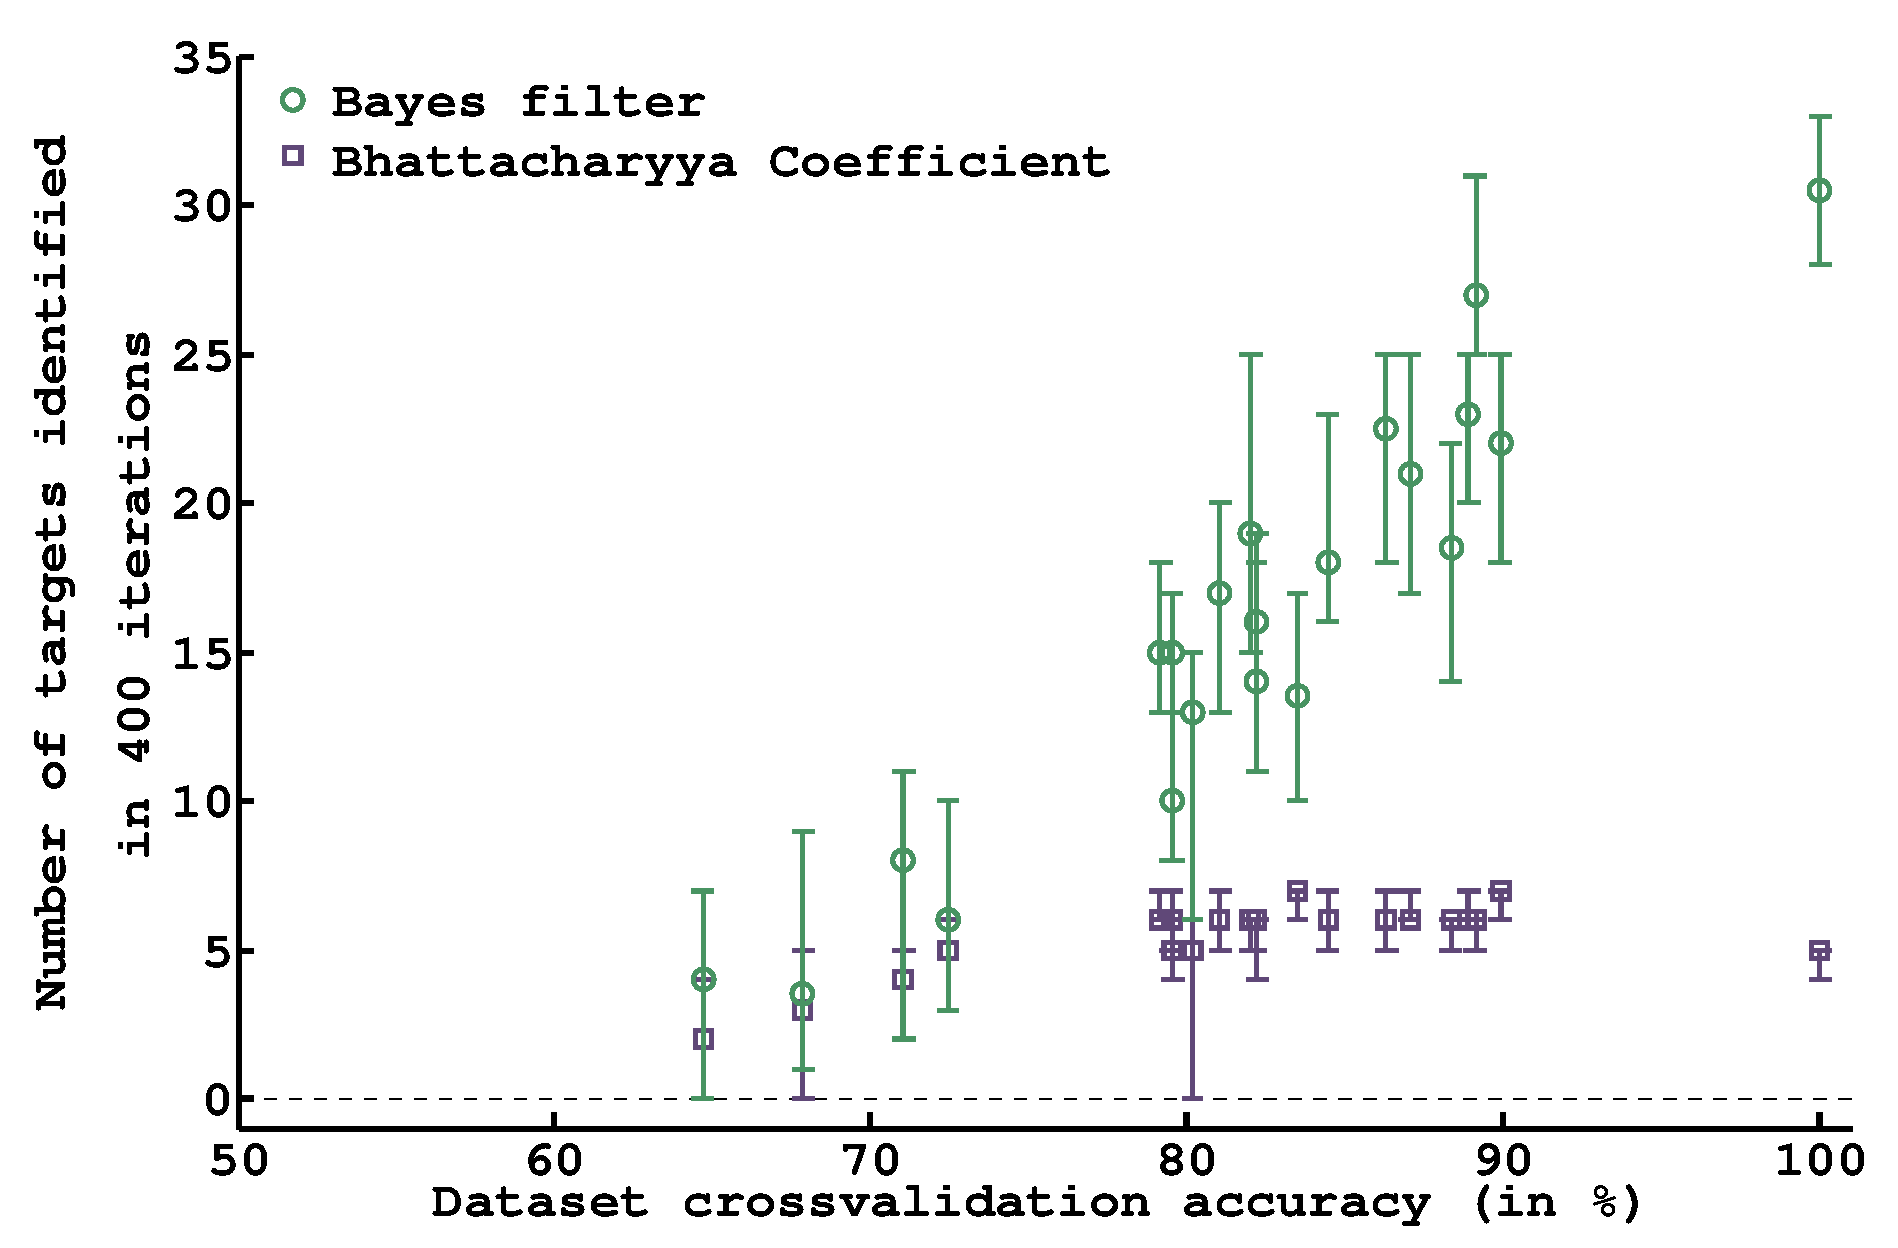
\includegraphics[width=\plotsize\columnwidth]{\imgpath/battacharyya/plot_bhattha_vs_bayes}
        \caption{Number of targets correctly identified in $400$ iterations (the markers show the median values and the error bars the $2.5$th and $97.5$th percentiles). Comparison between switching to a Bayes filter method after identification of a first target instead of keeping the estimation given by the Bhattacharyya coefficient. The Bayes filter allows for a faster identification.}
        \label{fig:bhatta}
\end{figure} 

Figure~\ref{fig:avg_sum_400} shows the number of tasks correctly and incorrectly identified in $400$ iterations. For datasets of good qualities, we are able to identify more than $20$ tasks in $400$ iterations without the need for a calibration procedure (recap that previous works needed between 300 and 600 examples for the calibration phase \cite{chavarriaga2010learning,iturrate2010single}). The number of correctly identified tasks is strongly correlated to the quality of the dataset.

\begin{figure}[!ht]
    \centering
    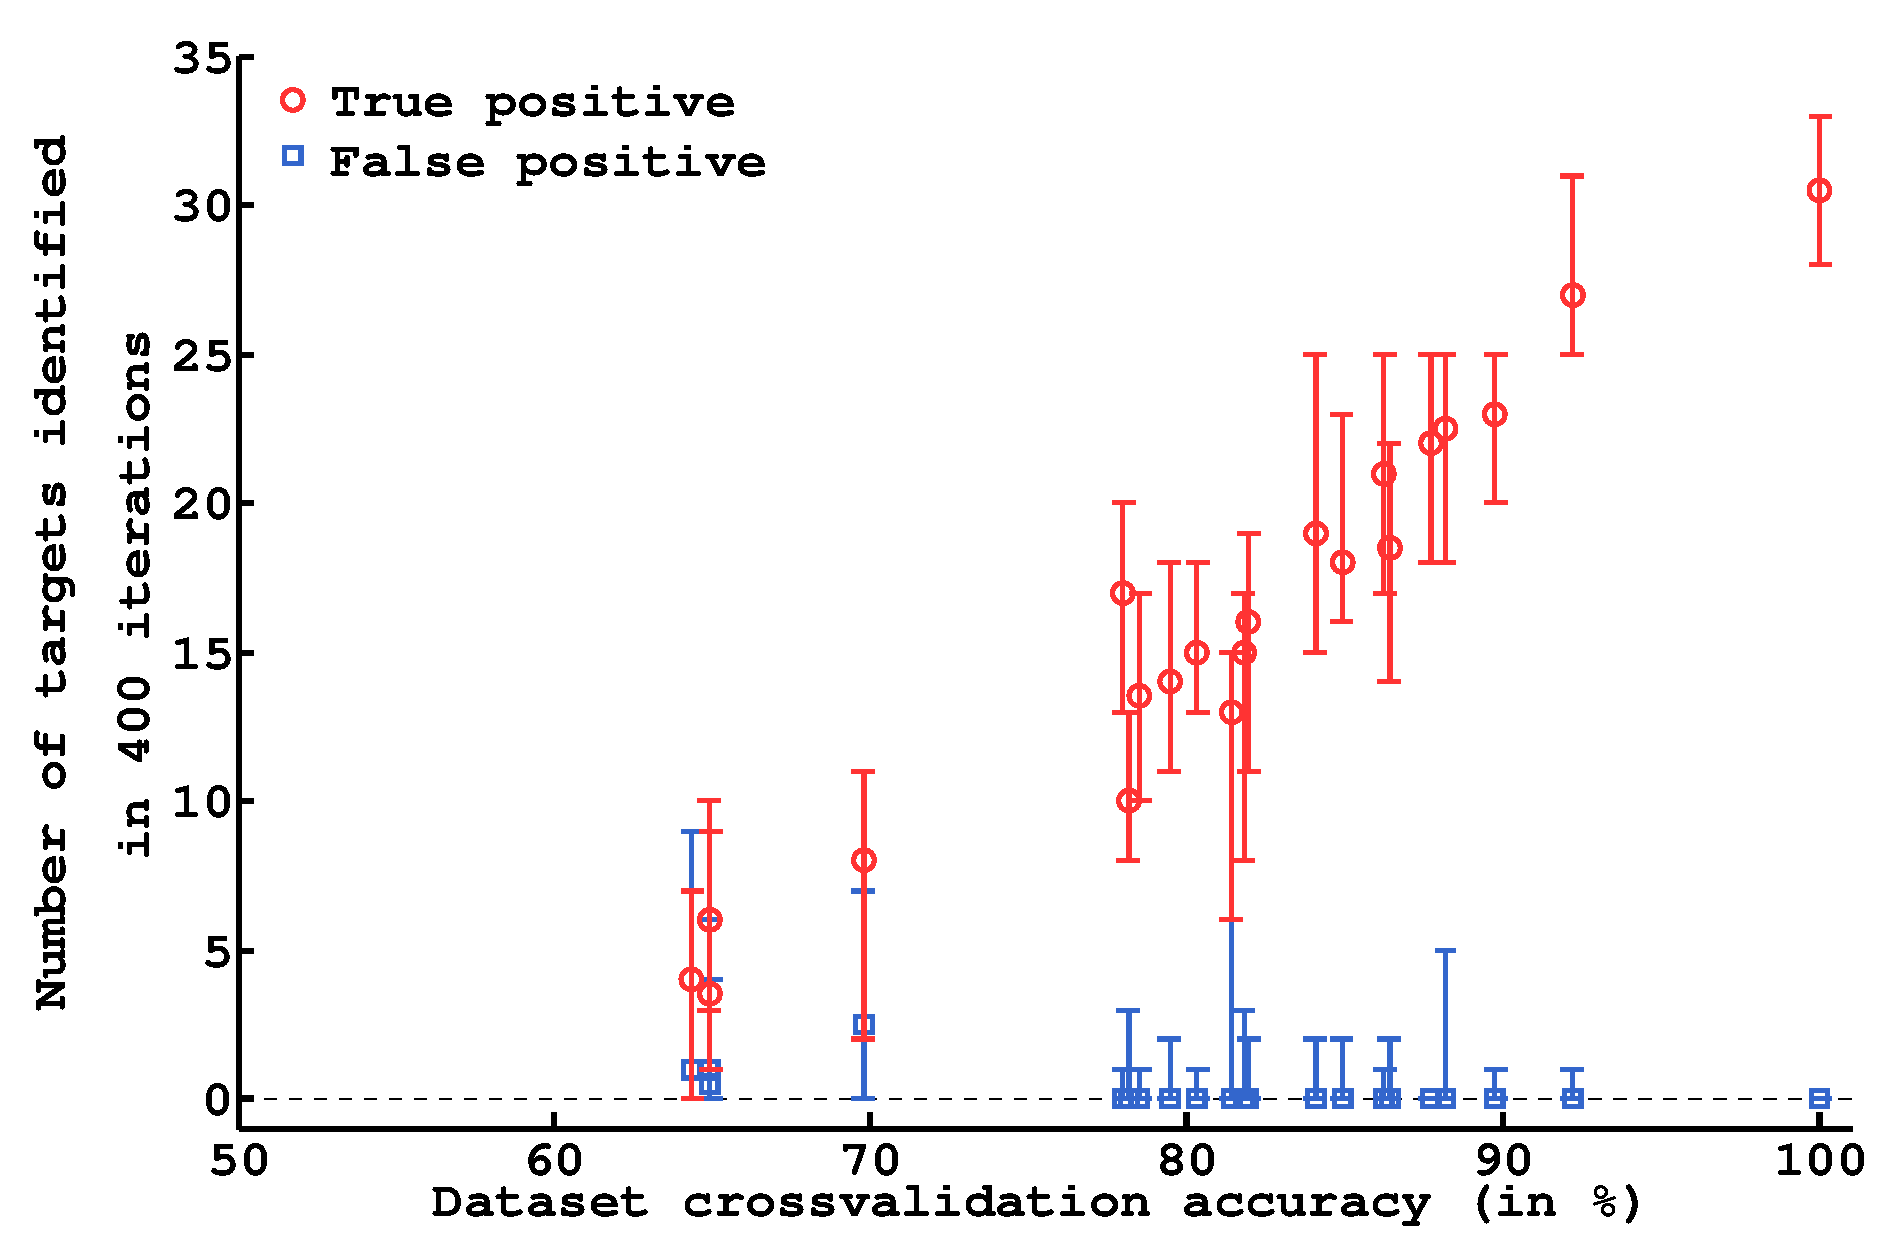
\includegraphics[width=\plotsize\columnwidth]{\imgpath/battacharyya/plot_first400_reach} 
    \caption{Number of targets correctly and incorrectly identified in $400$ iterations (the markers show the median values and the error bars the $2.5$th and $97.5$th percentiles). For datasets of good qualities, we are able to identify more than $20$ tasks in $400$ iterations without the need for a calibration procedure.}
    \label{fig:avg_sum_400}
\end{figure} 

\paragraph{Robustness to Abrupt Changes in the Signals' Properties }
\label{CenterRobustnessToAbruptChangesInTheSignalsProperties}

We now want to determine whether the system is robust to changes in the signals' properties that occur when we change between different problem settings \cite{iturrate2013task}. We modeled this by changing from $Ti$ to $Tj$ ($i \neq j$) after $400$ steps, and then executing $400$ more steps from $Tj$. Both combinations ($T1$ to $T2$ and $T2$ to $T1$) were tested.

Figure~\ref{fig:stage2} shows the number of tasks identified depending on the classification accuracy on $Tj$ when training a classifier from dataset $Ti$. For abrupt changes which conserve a classification accuracy above $70\%$ on the new signals, our method, based on a limited size prior, is able to recover and solve more than $20$ tasks in $400$ iterations. For those cases where the accuracy change is too drastic, starting from scratch may be a better solution than relying on the adaptation properties of our algorithm.

\begin{figure}[!ht]
    \centering
    \includegraphics[width=\plotsize\columnwidth]{\imgpath/battacharyya/plot_last400_reach}
    \caption{Number of targets correctly and incorrectly identified in $400$ iterations after an abrupt change in the signals properties (the markers show the median values and the error bars the $2.5$th and $97.5$th percentiles). For abrupt changes which conserve a classification accuracy above $70\%$ on the new signals, our method, based on a limited size prior, is able to recover and solve more than $20$ tasks in $400$ iterations.}
    \label{fig:stage2}
\end{figure}

\subsection{Online control}

This experiment evaluates if we can identify the task desired by the user even without an explicit calibration phase and without prior knowledge of the brain signals. The experiments were conducted with four subjects (aged between $25$ and $28$). Each subject was asked to mentally assess the agent's actions with respect to a given target. The system was not calibrated to decode the user EEG signals beforehand. Each subject performed $5$ runs, for each run a new target was randomly selected and provided to the user. There was an action every three seconds. Each run lasted $200$ actions, and the time between runs was around one minute.

The algorithm was able to identify the correct target for all runs of all the subjects, see Figure~\ref{fig:online_results}. There are strong variations among subjects but we note that our system identified each task in less iterations than a normal calibration phase requires (between 300 and 600 examples depending on the user performance \cite{chavarriaga2010learning,iturrate2010single}).

\begin{figure}[!htbp]
    \centering
    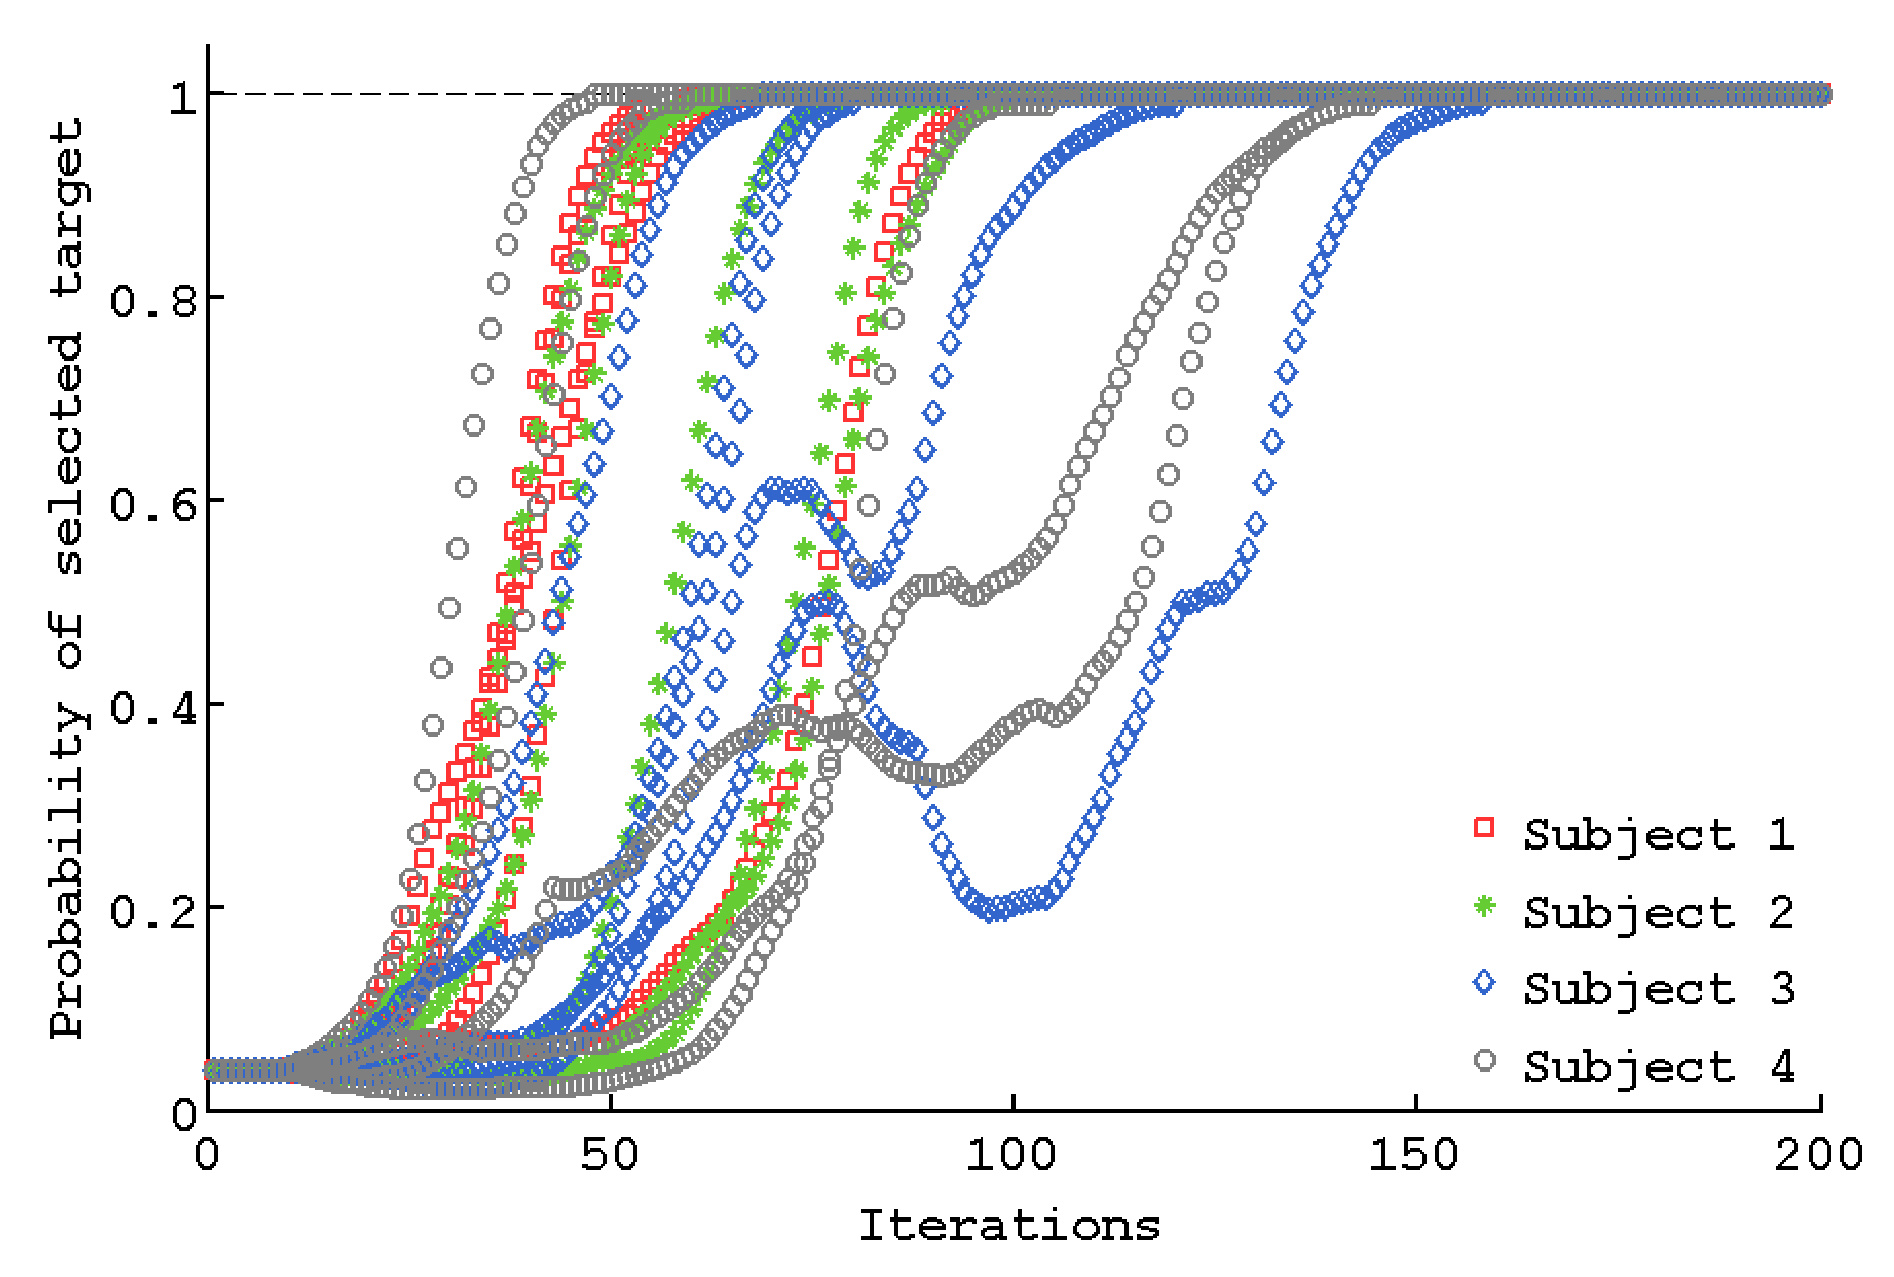
\includegraphics[width=\plotsize\columnwidth]{\imgpath/battacharyya/plot_realevolution}    
    \caption{Results from the online experiment: Evolution of the probability of the correct task for each subject and run. The algorithm was able to identify the correct target for each subjects and runs in less than 200 iterations.}
    \label{fig:online_results} 
\end{figure}

Table~\ref{ch6tab:steps} shows for each subject and run the number of iterations needed to reach the confidence threshold for the subject selected target.

On average, the number of iterations needed to identify the target was of 85 $\pm$ 32.

\begin{table}[!ht]
\centering
\begin{footnotesize}
\begin{tabular}{r|rrrrr|r}
    %\toprule
    & \textbf{Run1} & \textbf{Run2} & \textbf{Run3} & \textbf{Run4} & \textbf{Run5} & \textbf{mean$\pm$std} \\\hline
    %\midrule
    \textbf{S1} & 95 & 62 & 56 & 60 & 64 & 67 $\pm$ 16 \\
    \textbf{S2} & 89 & 77 & 98 & 60 & 62  & 77 $\pm$ 17 \\
    \textbf{S3} & 68 & 80 & 118 & 76 & 157 & 100 $\pm$ 37 \\
    \textbf{S4} & 98 & 142 & 57 & 142 & 47 & 97 $\pm$ 45 \\
    %\bottomrule
\end{tabular}
\end{footnotesize}
  \caption{Results from the online experiment: Number of iterations needed to identify the correct target for each subject and run. On average, the number of iterations needed to identify the target was of 85 $\pm$ 32.}
  \label{ch6tab:steps}
\end{table}

\subsection{Discussion}

We introduced a novel method for calibration-free BCI based control of sequential tasks with feedback signals. The method provides an unsupervised way to train a decoder with almost the same performance as state-of-the-art supervised classifiers, while keeping the system operational and solving the task requested by the user since the beginning. 
%
The intuition for our method is that the classification of the brain signals is easier when they are interpreted according to the task desired by the user. The method assumes a distribution of possible tasks and relies on finding which pair of decoder-task has the highest expected classification rate on the brain signals. 


The algorithm was tested with real online experiments, showing that the users were able to guide an agent to a desired position by mentally assessing the agent's actions and without any explicit calibration phase. Offline experiments show that we can identify an average of 20 tasks in 400 iterations without any calibration, while in previous works the calibration phase used between 300 and 600 examples. To improve the efficiency of the algorithm, we introduced a new planning method that uses the uncertainty in the decoder-task estimation. Finally, we analyzed the performance of the system in the presence of abrupt changes in the EEG signals. Our proposed method was able to adapt and reuse its learned models to the new signals. Furthermore, in those cases when the transfer is not possible, our method can still be used to recalibrate the system from scratch while solving the task.

A current limitation of the work is the need for a finite set of task hypotheses. This limitation could be solved by the use of a combination of particle filter and regularization on the task space. Additionally, our method can not dissociate fully symmetric hypotheses, e.g.\ right and left most state of our 1D grid world (Fig. \ref{fig:GM}), as the interpretation of feedback signals will also be symmetric and therefore as likely. This latter problem can be solved by redefining the set of hypotheses or the action set, for instance by adding a ``stop'' action valid only at the target state.

This work opens a new perspective regarding the global challenge of interacting with machines. It has application to many interaction problems which requires a machine to learn how to interpret unknown communicative signals. A promising avenue, outside the BCI field, lies in human robot interaction scenarios where robots must learn from, and interact with, many different users who have their own limitations and preferences.
